\documentclass[fontscale=0.38,a0paper]{baposter}

\tracingstats=2

\usepackage{times}
\usepackage{calc}
\usepackage{graphicx}
\usepackage{amsmath}
\usepackage{amssymb}
\usepackage{relsize}
\usepackage{multirow}
\usepackage{bm}
\usepackage{caption}
\usepackage[authoryear,round]{natbib}
\usepackage[hidelinks]{hyperref}

\usepackage{tabularx}
\usepackage{booktabs}

\usepackage{colortbl}

\usepackage{multicol}

%\usepackage{pgfbaselayers}
%\pgfdeclarelayer{background}
%\pgfdeclarelayer{foreground}
%\pgfsetlayers{background,main,foreground}


%\usepackage{tikz}
%\usetikzlibrary{arrows,backgrounds,patterns,matrix,shapes,fit,calc,shadows,plotmarks,decorations.pathmorphing,positioning,trees}

\renewcommand{\familydefault}{\sfdefault}
\usepackage{helvet}
\usepackage{bookman}
\usepackage{palatino}

% My stuff
\newcommand{\E}{\mathbb{E}}
\renewcommand{\P}{\mathbb{P}}
% end my stuff

\selectcolormodel{cmyk}

% \graphicspath{{images/}}

%%%%%%%%%%%%%%%%%%%%%%%%%%%%%%%%%%%%%%%%%%%%%%%%%%%%%%%%%%%%%%%%%%%%%%%%%%%%%%%%
%%%% Some symbols used in the text
%%%%%%%%%%%%%%%%%%%%%%%%%%%%%%%%%%%%%%%%%%%%%%%%%%%%%%%%%%%%%%%%%%%%%%%%%%%%%%%%
%\newcommand{\sub}[2]{\ensuremath{#1_{\textrm{#2}}}}
%\newcommand{\gen}[2]{\ensuremath{\textrm{#1}_{\textrm{#2}}}}


%%%%%%%%%%%%%%%%%%%%%%%%%%%%%%%%%%%%%%%%%%%%%%%%%%%%%%%%%%%%%%%%%%%%%%%%%%%%%%%%
% Multicol Settings
%%%%%%%%%%%%%%%%%%%%%%%%%%%%%%%%%%%%%%%%%%%%%%%%%%%%%%%%%%%%%%%%%%%%%%%%%%%%%%%%
\setlength{\columnsep}{1em}
\setlength{\columnseprule}{0mm} % no vertical line


%%%%%%%%%%%%%%%%%%%%%%%%%%%%%%%%%%%%%%%%%%%%%%%%%%%%%%%%%%%%%%%%%%%%%%%%%%%%%%%%
% Save space in lists. Use this after the opening of the list
%%%%%%%%%%%%%%%%%%%%%%%%%%%%%%%%%%%%%%%%%%%%%%%%%%%%%%%%%%%%%%%%%%%%%%%%%%%%%%%%
\newcommand{\compresslist}{
\setlength{\itemsep}{1pt}
\setlength{\parskip}{0pt}
\setlength{\parsep}{0pt}
}

%%%%%%%%%%%%%%%%%%%%%%%%%%%%%%%%%%%%%%%%%%%%%%%%%%%%%%%%%%%%%%%%%%%%%%%%%%%%%%
%%% Other Macros
%%%%%%%%%%%%%%%%%%%%%%%%%%%%%%%%%%%%%%%%%%%%%%%%%%%%%%%%%%%%%%%%%%%%%%%%%%%%%%
% \renewcommand{\labelenumi}{\alph{enumi})}
% \renewcommand{\theenumi}{\alph{enumi})}
\newcommand{\postercaption}[1]{\begin{minipage}{\linewidth}\center\smaller
  {#1}\end{minipage}}



%%%%%%%%%%%%%%%%%%%%%%%%%%%%%%%%%%%%%%%%%%%%%%%%%%%%%%%%%%%%%%%%%%%%%%%%%%%%%%
%%% Begin of Document
%%%%%%%%%%%%%%%%%%%%%%%%%%%%%%%%%%%%%%%%%%%%%%%%%%%%%%%%%%%%%%%%%%%%%%%%%%%%%%

\begin{document}

%%%%%%%%%%%%%%%%%%%%%%%%%%%%%%%%%%%%%%%%%%%%%%%%%%%%%%%%%%%%%%%%%%%%%%%%%%%%%%
%%% Here starts the poster
%%%---------------------------------------------------------------------------
%%% Format it to your taste with the options
%%%%%%%%%%%%%%%%%%%%%%%%%%%%%%%%%%%%%%%%%%%%%%%%%%%%%%%%%%%%%%%%%%%%%%%%%%%%%%

% Define some colors
\definecolor{silver}{cmyk}{0,0,0,0.3}
\definecolor{black}{cmyk}{0,0,0.0,1.0}
\definecolor{white}{cmyk}{0,0,0.0,0.0}
\definecolor{darkSilver}{cmyk}{0,0,0,0.1}

\definecolor{darkYellow}{cmyk}{0,0,1.0,0.5}
\definecolor{yellow}{cmyk}{0,0,0.9,0.0}
\definecolor{reddishyellow}{cmyk}{0,0.22,1.0,0.0}
\definecolor{lightyellow}{cmyk}{0,0,0.3,0.0}
\definecolor{lighteryellow}{cmyk}{0,0,0.1,0.0}
\definecolor{lightestyellow}{cmyk}{0,0,0.05,0.0}

\definecolor{DavisBlue}{cmyk}{1,0.56,0,0.34}
%    C = 100  M = 56  Y = 0 K = 34


\definecolor{HohenheimBlue}{cmyk}{1,0.5,0,0.45}
\definecolor{HohenheimLightLightBlue}{RGB}{243,250,255}
\definecolor{HohenheimLightBlue}{RGB}{215,221,235}
\definecolor{HohenheimDarkBlue}{RGB}{52,104,152}
\definecolor{darkCyan}{cmyk}{1,1,0,0.5}
\definecolor{cyan}{cmyk}{1,0,0,0.0}
\definecolor{lightcyan}{cmyk}{0.3,0,0,0.0}
\definecolor{lightercyan}{cmyk}{0.1,0,0,0.0}
\definecolor{lightestcyan}{cmyk}{0.05,0,0,0.0}



\typeout{Poster Starts}
%Define custom background
\background{
  \begin{tikzpicture}[remember picture,overlay]%
    \draw (current page.north west)+(-2em,2em) node[anchor=north west] {\includegraphics[height=\textheight]{silhouettes_background}};
  \end{tikzpicture}%
}

\newlength{\leftimgwidth}
\begin{poster}%
  % Poster Options
  {
  % Columns and Column spacing
  columns=3,
  colspacing=1.5em,
  % Background
  % background=user,
  background=shade-tb,
  % Poster header options
  eyecatcher=yes,
  posterheaderheight=0.15\textheight,
  % Format of textbox header
  headerborder=open,
  % headershape=small-rounded,
  headershape=roundedright,
  headershade=shade-tb,
  % headershade=plain,
  headerfont=\Large\textsf, %Sans Serif
  % Format of textbox
  boxborder=small-rounded,
  % boxborder=roundedleft,    
  boxshade=plain,
  linewidth=0.5pt,
  % Color style
  % bgColorOne=lightestcyan,
  % bgColorTwo=lightcyan,
  bgColorOne=white,
  bgColorTwo=white,
  % borderColor=cyan,
  borderColor=black,
  headerColorOne=DavisBlue,
  % headerColorOne=cyan,
  headerColorTwo=black,
  % headerFontColor=black,
  headerFontColor=white,
  % boxColorOne=lightercyan,
  boxColorOne=HohenheimLightLightBlue,
  boxColorTwo=white,
  % Show grid to help with alignment
  grid=no
  % grid=yes
  }
  % Eye Catcher
  {
  \makebox[15em][r]{%
    \begin{minipage}{15em}
       \hfill
       \includegraphics[width=15em]{tskit_logo} \\
    \end{minipage}
    }
  }
  % Title
  {\sf %Sans Serif
  %\bf% %bold  
  \vspace{0.5em}
     \textbf{\textcolor{DavisBlue}{Tree sequences \\ for fast genome simulation and analysis}}\vspace{0.5em}}
  % Authors
  {\sf %Sans Serif
    Peter Ralph$^{\ddagger}$ \\  \vspace{-1.0mm}
    {\small \textit{$\ddagger$ Mathematics and Biology, University of Oregon} }\\
    {\textbf{code:}  \url{https://github.com/tskit-dev} }\\
    \vspace{0.8em}
    {Related posters: Jerome Kelleher (tree sequences) and Phillip Messer (SLiM)}
    % {\textbf{paper:}  \url{https://www.biorxiv.org/content/early/2018/01/26/248500} }\\
  }
  % Project logo
  {
    \makebox[15em][r]{%
      \begin{minipage}{12em}
        \hfill
          \includegraphics[width=10em]{UOSignature-STK-BLK} \\
      \end{minipage}
    }
  }

  % Width of left inset image
%  \setlength{\leftimgwidth}{0.78em+0.0em}

%%%%%%%%%%%%%%%%%%%%%%%%%%%%%%%%%%%%%%%%%%%%%%%%%%%%%%%%%%%%%%%%%%%%%%%%%%%%%%
%%% Now define the boxes that make up the poster
%%%---------------------------------------------------------------------------
%%% Each box has a name and can be placed absolutely or relatively.
%%% The only inconvenience is that you can only specify a relative position 
%%% towards an already declared box. So if you have a box attached to the 
%%% bottom, one to the top and a third one which should be in between, you 
%%% have to specify the top and bottom boxes before you specify the middle 
%%% box.
%%%%%%%%%%%%%%%%%%%%%%%%%%%%%%%%%%%%%%%%%%%%%%%%%%%%%%%%%%%%%%%%%%%%%%%%%%%%%%

%%%%%%%%%%%%%%%%%%%%%%%%%%%%%%%%%%%%%%%%%%%%%%%%%%%%%%%%%%%%%%%%%%%%%%%%%%%%%%
\headerbox{Tree sequences: all the genealogies}{name=intro,column=0,row=0,span=1}{
%%%%%%%%%%%%%%%%%%%%%%%%%%%%%%%%%%%%%%%%%%%%%%%%%%%%%%%%%%%%%%%%%%%%%%%%%%%%%%

A \textbf{tree sequence} describes
the correlated sequence of genealogical trees
that say how a set of chromosomes are related.

\emph{Observations:}

\begin{itemize}

    \item The \emph{pedigree} plus crossover locations
        would give us the tree sequence for \emph{everyone, ever}.

    \item Much less can fully describe the history relevant to a \emph{sample} of genomes.

    \item This is equivalent to the Ancestral Recombination Graph (ARG).

\end{itemize}


\citet{kelleher2016efficient}
introduced the \textbf{tree sequence} data structure
for a fast coalescent simulator, \texttt{msprime}.
Updated in \citet{kelleher2018efficient}.

}
%%%%%%%%%%%%%%%%%%%%%%%%%%%%%%%%%%%%%%%%%%%%%%%%%%%%%%%%%%%%%%%%%%%%%%%%%%%%%%


%%%%%%%%%%%%%%%%%%%%%%%%%%%%%%%%%%%%%%%%%%%%%%%%%%%%%%%%%%%%%%%%%%%%%%%%%%%%%%
\headerbox{Tables: a data structure for tree sequences}{name=tables,column=0,span=1,below=intro}{
%%%%%%%%%%%%%%%%%%%%%%%%%%%%%%%%%%%%%%%%%%%%%%%%%%%%%%%%%%%%%%%%%%%%%%%%%%%%%%

    % We updated and generalized the data structure in \citet{kelleher2018efficient}:

    \begin{itemize}

        \item \textbf{Edges:}   Who inherits from who. \\
            \emph{Records:} interval (left, right); parent node; child node.

        \item \textbf{Nodes:}   The ancestors those happen in. \\
            \emph{Records:} time ago (of birth); individual.

        \item \textbf{Mutations:}   When state changes along the tree. \\
            \emph{Records:} site index; node index; derived state.

        \item \textbf{Sites:}   Where mutations fall on the genome. \\
            \emph{Records:} genomic position; root state.

        \item \textbf{Individuals:} Optional. Containers for polyploids. \\
            \emph{Records:} metadata; pointed to by nodes.

    \end{itemize}

    \begin{center}
        \includegraphics[width=0.75\textwidth]{storing_everyone}
    \end{center}

}
%%%%%%%%%%%%%%%%%%%%%%%%%%%%%%%%%%%%%%%%%%%%%%%%%%%%%%%%%%%%%%%%%%%%%%%%%%%%%%


%%%%%%%%%%%%%%%%%%%%%%%%%%%%%%%%%%%%%%%%%%%%%%%%%%%%%%%%%%%%%%%%%%%%%%%%%%%%%%
\headerbox{Example}{name=ex,column=0,below=tables}{
%%%%%%%%%%%%%%%%%%%%%%%%%%%%%%%%%%%%%%%%%%%%%%%%%%%%%%%%%%%%%%%%%%%%%%%%%%%%%%

    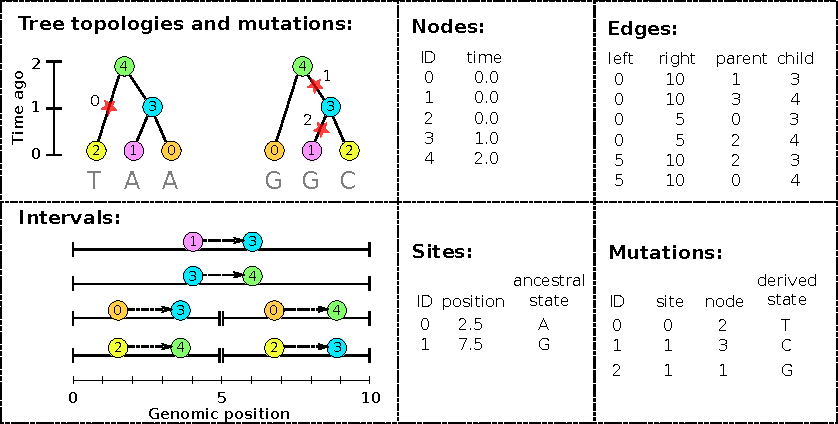
\includegraphics[width=\textwidth]{example_tree_sequence}

}
%%%%%%%%%%%%%%%%%%%%%%%%%%%%%%%%%%%%%%%%%%%%%%%%%%%%%%%%%%%%%%%%%%%%%%%%%%%%%%

%%%%%%%%%%%%%%%%%%%%%%%%%%%%%%%%%%%%%%%%%%%%%%%%%%%%%%%%%%%%%%%%%%%%%%%%%%%%%%
\headerbox{Another example}{name=ex2,column=0,below=ex}{
%%%%%%%%%%%%%%%%%%%%%%%%%%%%%%%%%%%%%%%%%%%%%%%%%%%%%%%%%%%%%%%%%%%%%%%%%%%%%%

    \noindent
    \tiny
\hfill
\begin{tabular}{|rr|}
  \hline
    \textbf{Nodes:} & \\
id & time \\ 
  \hline
  0 & 0.00 \\ 
    1 & 0.00 \\ 
    2 & 0.00 \\ 
    3 & 0.00 \\ 
    4 & 0.00 \\ 
    5 & 0.00 \\ 
    6 & 0.00 \\ 
    7 & 0.00 \\ 
    8 & 0.09 \\ 
    9 & 0.31 \\ 
   10 & 0.39 \\ 
   11 & 0.41 \\ 
   12 & 0.43 \\ 
   13 & 0.97 \\ 
   14 & 1.04 \\ 
   15 & 1.21 \\ 
   16 & 1.36 \\ 
   17 & 1.45 \\ 
   18 & 2.41 \\ 
   19 & 2.46 \\ 
   20 & 2.85 \\ 
   21 & 3.84 \\ 
   22 & 4.45 \\ 
   \hline
\end{tabular}
\hfill
\begin{tabular}{|rrrr|}
  \hline
    \textbf{Edges:} & & & \\
left & right & parent & child \\ 
  \hline
0.00 & 1.00 &   8 &   2 \\ 
  0.00 & 1.00 &   8 &   6 \\ 
  0.00 & 1.00 &   9 &   5 \\ 
  0.00 & 1.00 &   9 &   7 \\ 
  0.00 & 1.00 &  10 &   3 \\ 
  0.00 & 1.00 &  10 &   8 \\ 
  0.00 & 1.00 &  11 &   0 \\ 
  0.00 & 1.00 &  11 &   1 \\ 
  0.00 & 1.00 &  12 &   9 \\ 
  0.00 & 1.00 &  12 &  10 \\ 
  0.99 & 1.00 &  13 &   4 \\ 
  0.99 & 1.00 &  13 &  12 \\ 
  0.00 & 0.19 &  14 &  11 \\ 
  0.00 & 0.19 &  14 &  12 \\ 
  0.93 & 0.99 &  15 &   4 \\ 
  0.93 & 1.00 &  15 &  11 \\ 
  0.99 & 1.00 &  15 &  13 \\ 
  0.30 & 0.54 &  16 &   4 \\ 
  0.91 & 0.93 &  16 &   4 \\ 
  0.30 & 0.54 &  16 &  11 \\ 
  0.91 & 0.93 &  16 &  11 \\ 
  0.54 & 0.69 &  17 &   4 \\ 
   \hline
\end{tabular}
\begin{tabular}{|rrrr|}
  \hline
    \textbf{cont'd} & ... &  ... & ... \\
left & right & parent & child \\ 
  \hline
  0.54 & 0.69 &  17 &  12 \\ 
  0.69 & 0.91 &  18 &   4 \\ 
  0.69 & 0.91 &  18 &  11 \\ 
  0.00 & 0.30 &  19 &   4 \\ 
  0.69 & 0.69 &  19 &  11 \\ 
  0.19 & 0.46 &  19 &  12 \\ 
  0.69 & 0.99 &  19 &  12 \\ 
  0.00 & 0.19 &  19 &  14 \\ 
  0.93 & 0.99 &  19 &  15 \\ 
  0.30 & 0.46 &  19 &  16 \\ 
  0.91 & 0.93 &  19 &  16 \\ 
  0.69 & 0.69 &  19 &  17 \\ 
  0.69 & 0.91 &  19 &  18 \\ 
  0.19 & 0.30 &  20 &  11 \\ 
  0.19 & 0.30 &  20 &  19 \\ 
  0.60 & 0.69 &  21 &  11 \\ 
  0.60 & 0.69 &  21 &  17 \\ 
  0.54 & 0.60 &  22 &  11 \\ 
  0.46 & 0.54 &  22 &  12 \\ 
  0.46 & 0.54 &  22 &  16 \\ 
  0.54 & 0.60 &  22 &  17 \\ 
   \hline
\end{tabular}

}
%%%%%%%%%%%%%%%%%%%%%%%%%%%%%%%%%%%%%%%%%%%%%%%%%%%%%%%%%%%%%%%%%%%%%%%%%%%%%%



%%%%%%%%%%%%%%%%%%%%%%%%%%%%%%%%%%%%%%%%%%%%%%%%%%%%%%%%%%%%%%%%%%%%%%%%%%%%%%
\headerbox{References}{name=contrib,column=1,row=0}{
%%%%%%%%%%%%%%%%%%%%%%%%%%%%%%%%%%%%%%%%%%%%%%%%%%%%%%%%%%%%%%%%%%%%%%%%%%%%%%
  % \scriptsize
  \renewcommand{\section}[2]{\vskip 0.0em}
  \bibliographystyle{abbrvnat}
  \setlength{\bibsep}{0.0pt}
  \bibliography{refs}
}
%%%%%%%%%%%%%%%%%%%%%%%%%%%%%%%%%%%%%%%%%%%%%%%%%%%%%%%%%%%%%%%%%%%%%%%%%%%%%%


%%%%%%%%%%%%%%%%%%%%%%%%%%%%%%%%%%%%%%%%%%%%%%%%%%%%%%%%%%%%%%%%%%%%%%%%%%%%%%
\headerbox{Record history in forwards simulations?}{name=forwards,column=1,below=contrib}{
%%%%%%%%%%%%%%%%%%%%%%%%%%%%%%%%%%%%%%%%%%%%%%%%%%%%%%%%%%%%%%%%%%%%%%%%%%%%%%


    \begin{itemize}

        \item Coalescent simulations are \emph{much faster}
            than forwards-time, individual-based simulations
            because they don't have to keep track of \emph{everyone},
            only the ancestors of your sample.

        \item \textbf{But:} selection, or sufficient geographic structure,
            break the assumptions of coalescent theory.

        \item If we \emph{record the tree sequence}
            that relates everyone to everyone else,
            after the simulation is over we can put neutral mutations down on the trees.

        \item Since neutral mutations don't affect demography,
            this is \emph{equivalent} to having kept track of them throughout.

        \item This means recording the entire genetic history of \textbf{everyone} in the population, \textbf{ever}.

    \end{itemize}

}
%%%%%%%%%%%%%%%%%%%%%%%%%%%%%%%%%%%%%%%%%%%%%%%%%%%%%%%%%%%%%%%%%%%%%%%%%%%%%%


%%%%%%%%%%%%%%%%%%%%%%%%%%%%%%%%%%%%%%%%%%%%%%%%%%%%%%%%%%%%%%%%%%%%%%%%%%%%%%
\headerbox{How to do it}{name=howfwd,column=1,below=forwards}{
%%%%%%%%%%%%%%%%%%%%%%%%%%%%%%%%%%%%%%%%%%%%%%%%%%%%%%%%%%%%%%%%%%%%%%%%%%%%%%

    \begin{enumerate}

        \item Add new individuals and their chromosomes to the Individual and Node Tables, respectively.
        \item Record in the Edge Table 
            which parental chromosome each gamete inherited each bit of genome from.
        \item Add any new selected mutations to the Mutation Table 
            and (if necessary) their locations to the Site Table.

    \end{enumerate}

\includegraphics[width=7em]{../finger_right} 
\parbox[bottom]{20em}{
    \vspace{-4em}
    {\Large \emph{This is too much data.}} \\
    \emph{\ldots but,} most of it can be \emph{simplified} away.
}

}
%%%%%%%%%%%%%%%%%%%%%%%%%%%%%%%%%%%%%%%%%%%%%%%%%%%%%%%%%%%%%%%%%%%%%%%%%%%%%%



%%%%%%%%%%%%%%%%%%%%%%%%%%%%%%%%%%%%%%%%%%%%%%%%%%%%%%%%%%%%%%%%%%%%%%%%%%%%%%
\headerbox{Simulations, $50\times$ faster}{name=fast,column=1,below=howfwd}{
%%%%%%%%%%%%%%%%%%%%%%%%%%%%%%%%%%%%%%%%%%%%%%%%%%%%%%%%%%%%%%%%%%%%%%%%%%%%%%

    Recording, simplifying, and output of tables, is done with \texttt{C} code in \texttt{tskit}.

    % The simulation was done in \texttt{fwdpp} (C++ by Kevin Thornton),
    % connected with \texttt{pybind11} and \texttt{numpy}.
    % \textit{Machine:} Ubuntu / 2x 2.6 GHz Intel E5-2650 CPU.

    % \emph{Simulation parameters:}
    % \begin{itemize}
    %         \compresslist
    %     \item  Wright-Fisher population of size $N$, for $10N$ generations
    %     \item  neutral mutation rate $\mu$ equal to recombination rate $r$ per gamete
    %     \item  many, weakly deleterious mutations: rate $\mu/100$ with
    %         $s$ exponentially distributed with mean $2.5/N$.
    % \end{itemize}

    \begin{center}
    % 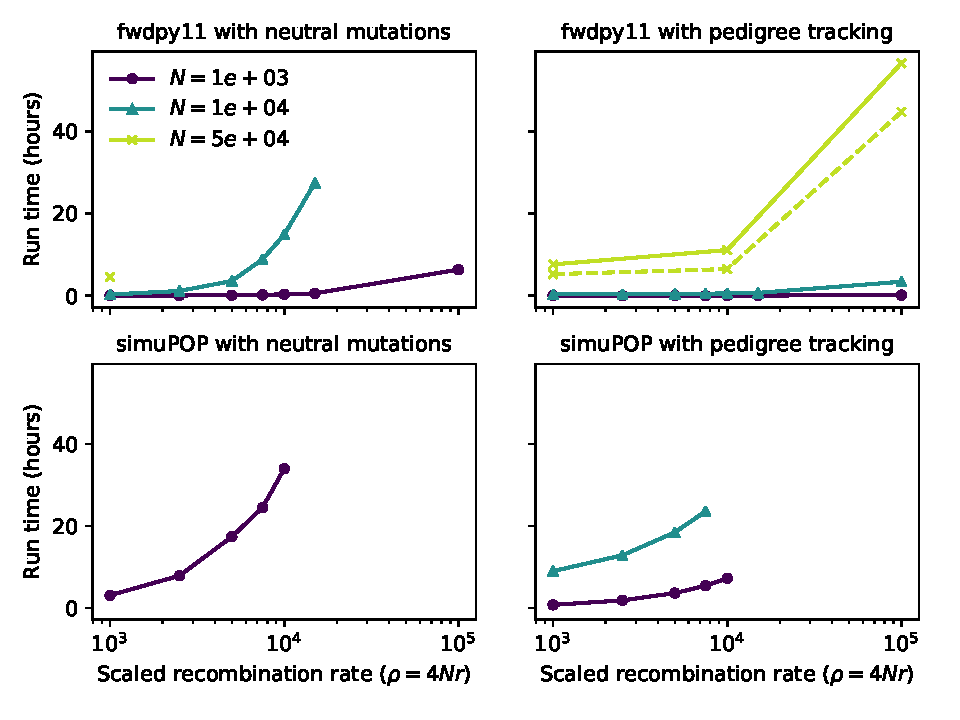
\includegraphics[width=\textwidth]{rawspeed}

    \parbox[bottom]{0.49\textwidth}{
        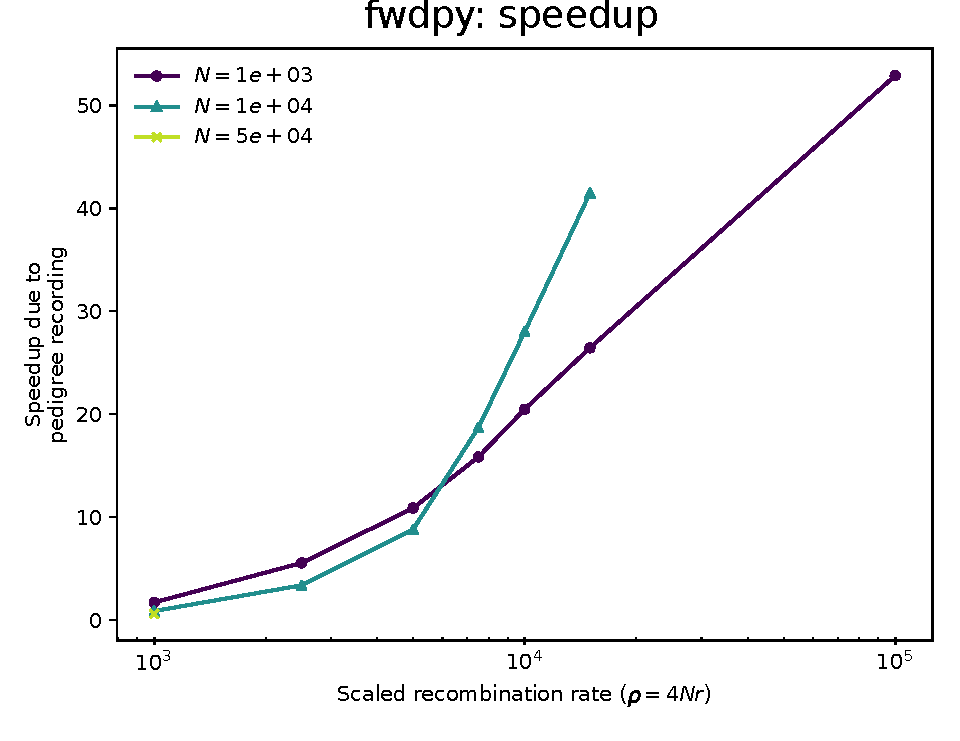
\includegraphics[width=0.45\textwidth]{speedup}
        (above) many selected mutations;
        (right) neutral.
    }
    \parbox[bottom]{0.49\textwidth}{
        \includegraphics[width=0.45\textwidth]{slim_speed}
    }
    \end{center}

    Simulations that recorded tree sequences
    had neutral mutation rate set to zero during the simulation,
    and neutral mutations added \emph{afterwards}.
    
    \vspace{2em}

    Results in \citet{haller2018treesequence,kelleher2018efficient}.
    
    \vspace{2em}

    {\Large
    Now in SLiM and fwdpp!
    }

}
%%%%%%%%%%%%%%%%%%%%%%%%%%%%%%%%%%%%%%%%%%%%%%%%%%%%%%%%%%%%%%%%%%%%%%%%%%%%%%


%%%%%%%%%%%%%%%%%%%%%%%%%%%%%%%%%%%%%%%%%%%%%%%%%%%%%%%%%%%%%%%%%%%%%%%%%%%%%%
\headerbox{A general class of statistics}{name=stats,column=2,row=0}{
%%%%%%%%%%%%%%%%%%%%%%%%%%%%%%%%%%%%%%%%%%%%%%%%%%%%%%%%%%%%%%%%%%%%%%%%%%%%%%

        Every single-site statistic is a function from genotype patterns to $\mathbb{R}$,
        and each SNP genotype pattern is determined by 
            the samples below the edge it occurs on.
            \vspace{1em}

    \emph{Ingredients:}
    \begin{enumerate}
            \compresslist
        \item A list of $k$ subsets of samples, $I_1, \ldots, I_k$,
            with $|I_j| = N_j$.
        \item A weighting function $f : \mathbb{N}^k \to \mathbb{R}$.
    \end{enumerate}

    \emph{Computation} on a genome of length $L$ with with $M$ SNPs:
    \begin{enumerate}
            \compresslist
        \item Let $n_i(j)$ be the number of samples in $I_j$
            that inherit mutation $i$.
        \item Use the weighting function to compute the weight of each mutation;
            average these across the genome:
            \[
                S(w) := \dfrac{1}{L} \sum_{i=1}^M (w(n_1, \ldots, n_k)  
                                        + w(N_1 - n_1, \ldots, N_k - n_k) .
            \]
    \end{enumerate}

}
%%%%%%%%%%%%%%%%%%%%%%%%%%%%%%%%%%%%%%%%%%%%%%%%%%%%%%%%%%%%%%%%%%%%%%%%%%%%%%


%%%%%%%%%%%%%%%%%%%%%%%%%%%%%%%%%%%%%%%%%%%%%%%%%%%%%%%%%%%%%%%%%%%%%%%%%%%%%%
\headerbox{Examples}{name=examples,column=2,below=stats}{
%%%%%%%%%%%%%%%%%%%%%%%%%%%%%%%%%%%%%%%%%%%%%%%%%%%%%%%%%%%%%%%%%%%%%%%%%%%%%%

    Folded SFS:
        $$ f_\ell(n_1) = \textbf{1}_\ell(n_1) \qquad \text{for}\; 1 \le \ell \le N_1 - 1 .$$

    Divergence between $I_1$ and $I_2$:
        $$ w(n_1, n_2) = n_1 (N_2 - n_2) / N_1 N_2 .$$

    Patterson's $f_4(I_1, I_2; I_3, I_4)$:
        \begin{align*}
           &w(n_1, n_2, n_3, n_4) \\
            & \qquad =
            \frac{
               n_1 n_3 (N_2 - n_2) (N_4 - n_4)
                      - n_1 n_4 (N_2 - n_2) (N_3 - n_3) }{ N_1 N_2 N_3 N_4  }
              .  \end{align*}

}

%%%%%%%%%%%%%%%%%%%%%%%%%%%%%%%%%%%%%%%%%%%%%%%%%%%%%%%%%%%%%%%%%%%%%%%%%%%%%%
\headerbox{Computation}{name=computation,column=2,below=examples}{
%%%%%%%%%%%%%%%%%%%%%%%%%%%%%%%%%%%%%%%%%%%%%%%%%%%%%%%%%%%%%%%%%%%%%%%%%%%%%%

    \begin{enumerate}
            \compresslist
        \item[0.]
            Find $n$ for each node in the first tree.
        \item[1.]
            Compute $f(n)$ for each mutation on this tree,
            and add these to the total.
        \item[2.]
            Update the tree, and update $n$ for each node
            in the path from changed nodes to the root.
        \item[3.]
            Return to (1).
        \item[4.]
            When done, divide the total by the sequence length.
    \end{enumerate}

    \emph{Complexity} for $N$ samples at $L$ SNPs with $T$ trees:
        $$ O(N + L + T \log(N)) . $$
    This is much better than using the genotype matrix, which is $O(NL)$.

}

%%%%%%%%%%%%%%%%%%%%%%%%%%%%%%%%%%%%%%%%%%%%%%%%%%%%%%%%%%%%%%%%%%%%%%%%%%%%%%
\headerbox{Other notes}{name=other,column=2,below=computation}{
%%%%%%%%%%%%%%%%%%%%%%%%%%%%%%%%%%%%%%%%%%%%%%%%%%%%%%%%%%%%%%%%%%%%%%%%%%%%%%
    \begin{itemize}
        \item 
            The \emph{same} statistics can be computed 
            as weighted averages of \textbf{branch lengths} also,
            which gives the expected value of the statistic, averaged over mutational noise.

        \item 
            This tracks who is ancestral to a set of samples;
            \emph{a dual procedure} tracks who has inherited from a set of ancestors.

        \item
            \emph{Many statistics} can be computed on the same pass through the tree sequence
            with little additional cost.

        \item
            The implementation computes these in \emph{windows}.

    \end{itemize}
}

%%%%%%%%%%%%%%%%%%%%%%%%%%%%%%%%%%%%%%%%%%%%%%%%%%%%%%%%%%%%%%%%%%%%%%%%%%%%%%
\headerbox{Updating internal state}{name=statfig,column=2,below=other}{
%%%%%%%%%%%%%%%%%%%%%%%%%%%%%%%%%%%%%%%%%%%%%%%%%%%%%%%%%%%%%%%%%%%%%%%%%%%%%%

    \includegraphics[width=0.3\textwidth]{stats_1}
    \includegraphics[width=0.3\textwidth]{stats_2}
    \includegraphics[width=0.3\textwidth]{stats_3}

}


%%%%%%%%%%%%%%%%%%%%%%%%%%%%%%%%%%%%%%%%%%%%%%%%%%%%%%%%%%%%%%%%%%%%%%%%%%%%%%
\headerbox{}{name=trees,column=0,above=bottom,span=3}{
%%%%%%%%%%%%%%%%%%%%%%%%%%%%%%%%%%%%%%%%%%%%%%%%%%%%%%%%%%%%%%%%%%%%%%%%%%%%%%

    \includegraphics[width=0.085\textwidth]{tree0}
    \includegraphics[width=0.085\textwidth]{tree1}
    \includegraphics[width=0.085\textwidth]{tree2}
    \includegraphics[width=0.085\textwidth]{tree3}
    \includegraphics[width=0.085\textwidth]{tree4}
    \includegraphics[width=0.085\textwidth]{tree5}
    \includegraphics[width=0.085\textwidth]{tree6}
    \includegraphics[width=0.085\textwidth]{tree7}
    \includegraphics[width=0.085\textwidth]{tree8}
    \includegraphics[width=0.085\textwidth]{tree9}
    \includegraphics[width=0.085\textwidth]{tree10}


}
%%%%%%%%%%%%%%%%%%%%%%%%%%%%%%%%%%%%%%%%%%%%%%%%%%%%%%%%%%%%%%%%%%%%%%%%%%%%%%

\end{poster}%
\end{document}


%%%%%%%%%%%%%%%%%%%%%%%%%%%%%%%%%%%%%%%%%%%%%%%%%%%%%%%%%%%%%%%%%%%%%%%%%%%%%%
\headerbox{Simplification}{name=simplify,column=1,below=howfwd}{
%%%%%%%%%%%%%%%%%%%%%%%%%%%%%%%%%%%%%%%%%%%%%%%%%%%%%%%%%%%%%%%%%%%%%%%%%%%%%%

    Given an input tree sequence
    and a subset of its nodes (the \emph{samples}),
    we want a new tree sequence for which:

    \begin{enumerate}
        \item All marginal trees match the corresponding subtree 
            in the input tree sequence.

        \item Every non-sample node in marginal trees has at least two children.

        \item All nodes and edges ancestral to at least one sample.

        \item No adjacent redundant edges \\
            (e.g., $(\ell, x, p, c) + (x, r, p, c) \rightarrow (\ell, r, p, c)$).
    \end{enumerate}


    To simplify a tree sequence
    to the history of the \emph{samples},
    we:

    \begin{itemize}
        \item Paint each \emph{sampled} chromosome a distinct color.

        \item Moving back up the tree sequence,
            copy colors of each chromosome to the parental chromosomes
            they inherited from.

        \item If two colors go in the same spot (\emph{coalescence}),
            replace with a new color (unique to that ancestor).
            Output a node for the ancestor and an edge for the coalescence.

        \item Once all colors have coalesced in a given segment,
            stop propagating it.
    \end{itemize}

}
%%%%%%%%%%%%%%%%%%%%%%%%%%%%%%%%%%%%%%%%%%%%%%%%%%%%%%%%%%%%%%%%%%%%%%%%%%%%%%


%%%%%%%%%%%%%%%%%%%%%%%%%%%%%%%%%%%%%%%%%%%%%%%%%%%%%%%%%%%%%%%%%%%%%%%%%%%%%%
\headerbox{Summary}{name=summary,column=2,below=stats}{
%%%%%%%%%%%%%%%%%%%%%%%%%%%%%%%%%%%%%%%%%%%%%%%%%%%%%%%%%%%%%%%%%%%%%%%%%%%%%%

    Tree sequences 
    \begin{itemize}
        \item \ldots can make your simulations much faster
        \item \emph{because} they record genealogical history.
        \item (And, then you have genealogies!)
        \item \ldots can store genomic data \emph{very} efficiently,
        \item and compute with genomic data \emph{very} quickly.
    \end{itemize}

    \emph{Why} are they so useful?
    It is a compression scheme, provided by the process itself that produced the data.
    \emph{(think: optimal compression into shared haplotypes)}

}
%%%%%%%%%%%%%%%%%%%%%%%%%%%%%%%%%%%%%%%%%%%%%%%%%%%%%%%%%%%%%%%%%%%%%%%%%%%%%%

